\chapter{Transformada de Fourier}{\label{trans_Fourier}} %Passagem do discreto para o contínuo. Definição.
A série de Fourier é uma ferramenta para representar funções periódicas. Como os problemas de interesse podem envolver fun\c{c}\~{o}es n\~{a}o peri\'{o}dicas, neste cap\'{i}tulo definiremos uma representa\c{c}\~{a}o para essas fun\c{c}\~{o}es que possuem interpreta\c{c}\~{a}o como extens\~{a}o do conceito de s\'{e}rie de Fourier.
\section{Passagem do discreto para o contínuo}
Podemos construir uma representação em séries de Fourier para um função $f(t)$ não-periódica sempre que nos restringimos a um intervalo finito $[-T/2,T/2]$, isto é, construímos a função $f_T(t)$ T-periódica que coincide com $f(t)$ no intervalo citado:
\begin{equation}{\label{T-period}}\begin{array}{rcll}
 f_T(t)&=&f(t),&-T/2\leq t<T/2\\
 f_T(t+T)&=&f_T(t),&\forall t\in \mathbb{R}
 \end{array}
\end{equation}
\begin{ex}{\label{ex_Transf_1}} Considerando a função $f(t)=e^{-|t|}$, definimos funções $f_T(t)$ como na equação (\ref{T-period}) e apresentamos os gráficos de $f(t)$ e $f_T(t)$ para $T=2$ e $T=4$ na figura \ref{fig_T_tenda}.
\begin{figure}[!ht]
\begin{center}

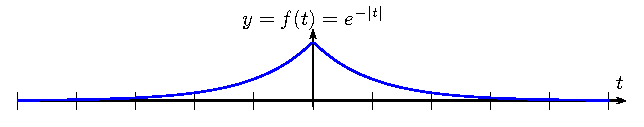
\includegraphics{cap_transformada_de_fourier/pics/figura_1}
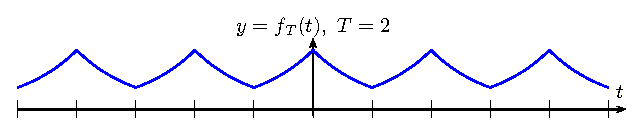
\includegraphics{cap_transformada_de_fourier/pics/figura_2}
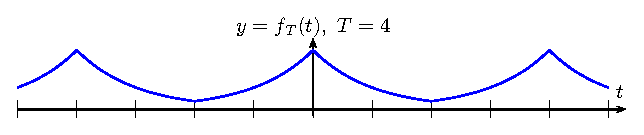
\includegraphics{cap_transformada_de_fourier/pics/figura_3}\end{center}
\caption{\label{fig_T_tenda}}
\end{figure}
Observe que a função $f_T(t)$ carrega consigo informação sobre a função $f(t)$. Naturalmente, gostaríamos de poder obter o limite $T\to \infty$, a fim de aproximar $f_T(t)$ tanto quando possível de $f(t)$. Como $T$ representa o período da função $f_T(t)$, quando $T$ cresce a frequência fundamental $w_F$ descresce. A função $f_T(t)$ possui série de Fourier da forma
$$
f_T(t)=\sum_{n=-\infty}^\infty C_n e^{iw_n t},
$$
onde
\begin{eqnarray}
 \nonumber C_n&=&\frac{1}{T}\int_{-T/2}^{T/2}e^{-|t|}e^{-iw_nt}dt = \frac{1}{T}\int_{-T/2}^{T/2}e^{-|t|}\left(\cos(w_nt)-i\sen(w_nt)\right)dt\\
 \nonumber &=&\frac{2}{T}\int_{0}^{T/2}e^{-|t|}\cos(w_nt)dt= \frac{2}{T}\int_{0}^{T/2}e^{-t}\cos(w_nt)dt\\
 \nonumber &=&\frac{2}{T}\left[\frac{ w_n \sen(t w_n)-\cos(t w_n)}{w_n^2+1}e^{-t}\right]_0^{T/2}\\
 \nonumber &=&\frac{2}{T}\frac{ \left[w_n \sen\left(\frac{Tw_n}{2}\right)-\cos\left(\frac{Tw_n}{2}\right)\right]e^{-\frac{T}{2}}+1}{w_n^2+1}\\
 \nonumber &=&\frac{2}{T}\frac{ \left[w_n \sen\left(n\pi\right)-\cos\left(n\pi\right)\right]e^{-\frac{T}{2}}+1}{w_n^2+1}\\
&=&\frac{2}{T}\frac{ 1-(-1)^ne^{-\frac{T}{2}}}{w_n^2+1}      {\label{TCn}}
 \end{eqnarray}
Observemos os diagramas de especto para $f_T(t)$ multiplicado por $T$ quando $T=2$, $T=4$ e $T=8$ na figura \ref{dia_espc_tenda}.
 \begin{figure}[!ht]

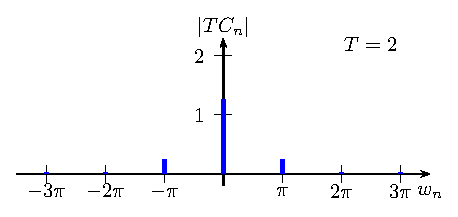
\includegraphics{cap_transformada_de_fourier/pics/figura_4}
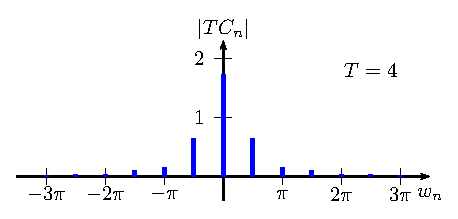
\includegraphics{cap_transformada_de_fourier/pics/figura_5}
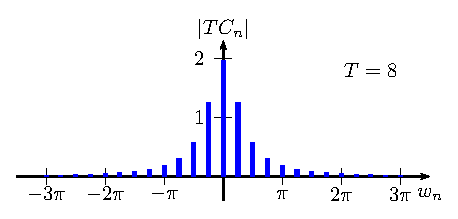
\includegraphics{cap_transformada_de_fourier/pics/figura_6}\caption{\label{dia_espc_tenda}}
\end{figure}
 \end{ex}
Como a distância entre duas raias espectrais é igual a frequência fundamental $w_F=w_1$, a densidade de raias aumenta, tornando mais densa na reta. A serie de Fourier da função $f_T(t)$ é dada por
$$
f_T(t)=\sum_{n=-\infty}^\infty C_n e^{i w_n t},
$$
onde 
$$C_n=\frac{1}{T}\int_{-T/2}^{T/2}f_T(\tau)e^{-iw_n \tau}d\tau=\frac{1}{T}\int_{-T/2}^{T/2}f(\tau)e^{-iw_n \tau}d\tau.$$
Definimos agora a função $$F_T(w)=\int_{-T/2}^{T/2}f(\tau)e^{-iw \tau}d\tau$$ e escrevemos $f_T(t)$ em termos de $F_T(w)$:
\begin{eqnarray}
\nonumber f_T(t)&=&\sum_{n=-\infty}^\infty \frac{1}{T}F_T(w_n) e^{i w_n t}\\&=& \sum_{n=-\infty}^\infty \frac{w_F}{2\pi}F_T(w_n) e^{i w_n t}
\\\nonumber &=& \sum_{n=-\infty}^\infty \frac{\Delta w}{2\pi}F_T(w_n) e^{i w_n t}
\\{\label{f_T}}&=&\frac{1}{2\pi} \sum_{n=-\infty}^\infty F_T(w_n) e^{i w_n t}\Delta w
\end{eqnarray}
Observe que a função $F_T(w)$ converge para cada frequência $w$ para a função 
$$
F(w)=\int_{-\infty}^\infty f(t) e^{-iw t}dt.
$$
Fazendo $T\to \infty$, a soma a direita na equação (\ref{f_T}) é uma soma de Riemann que converge para uma integral:
$$
f(t)=\frac{1}{2\pi} \int_{-\infty}^\infty F(w)e^{iw t}dw,
$$
onde
$$F(w)=\int_{-\infty}^{\infty}f(t)e^{-i w t}dt$$
\begin{ex} Continuamos com o exemplo \ref{ex_Transf_1}. Dada a função $f(t)=e^{-|t|}$, podemos escrever
$$
f(t)=\frac{1}{2\pi} \int_{-\infty}^\infty F(w)e^{iw t}dw,
$$
onde
\begin{eqnarray*}
F(w)&=&\lim_{T\to\infty}\int_{-T/2}^{T/2}e^{-|t|} e^{-i w t}dt\\
&=&\lim_{T\to\infty}\left(2\frac{ (-1)^ne^{-\frac{T}{2}}+1}{w^2+1} \right)\\
&=&\frac{2}{w^2+1},
\end{eqnarray*}
onde usamos a expressão para $TC_n$ dada por (\ref{TCn}). De fato, usando uma tabela de integrais (ou método dos resíduos), temos
\begin{eqnarray}
\frac{1}{2\pi} \int_{-\infty}^\infty \frac{2}{w^2+1} \cos(wt)dw
&=&\frac{1}{\pi} \int_{0}^\infty \frac{1}{w^2+1} \cos(wt)dw\\
&=&e^{-|t|}
\end{eqnarray}
\end{ex}
\section{Transformada de Fourier}
\begin{defn}Seja $f(t)$ uma função real (ou complexa), define-se a transformada de Fourier $F(w)$ de $f(t)$ como:
$$
F(w)=\mathcal{F}\{f(t)\}=\int_{-\infty}^\infty f(t)e^{-iwt}dt.
$$
\end{defn}
\begin{defn}Seja $F(w)$ uma função real (ou complexa), define-se a transformada inversa de Fourier $f(t)$ de $F(w)$ como:
$$
f(t)=\mathcal{F}^{-1}\{F(w)\}=\frac{1}{2\pi}\int_{-\infty}^\infty F(w)e^{iwt}dw.
$$
\end{defn}
\begin{obs}É costumeiro em Física e Engenharia usar a variável $k$ na transformada de Fourier de função em $x$, isto é,
\begin{eqnarray*}
F(k)&=&\mathcal{F}\{f(x)\}=\int_{-\infty}^\infty f(x)e^{-ikx}dx\\
f(x)&=&\mathcal{F}^{-1}\{F(k)\}=\frac{1}{2\pi}\int_{-\infty}^\infty F(k)e^{ikx}dk.
\end{eqnarray*}
Os pares de variáveis $t$-$w$ e $x$-$k$ são chamados de pares de variáveis recíprocas. A letra $k$ é o número de onda, conceito análogo no espaço ao conceito de frequência angular no tempo, isto é, enquanto $w=\frac{2\pi}{T}$, $k=\frac{2\pi}{\lambda}$, onde $\lambda$ é o comprimento de onda.	
\end{obs}
\begin{ex} Seja 
$$f(t)=\left\{\begin{array}{cc}e^{at}&\hbox{se}\ t<0\\
e^{-bt}&\hbox{se}\ t>0
\end{array}\right.
$$
onde $a$ e $b$ são constantes positivas. A figura \ref{fig_trans_1} mostra o gráfico de $f(t)$ para $a=1$ e $b=3$.
\begin{figure}[!ht]
\begin{center}

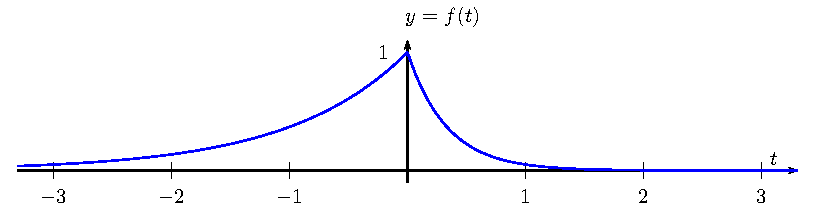
\includegraphics{cap_transformada_de_fourier/pics/figura_7}\end{center}
\caption{\label{fig_trans_1} Gráfico de $f(t)=e^{t}$, se $t<0$ ou $f(t)=e^{-3t}$ se $t>0$.  }
\end{figure}
A transformada de Fourier de $f(t)$ é calculada da seguinte forma:
\begin{eqnarray*}
F(w)=\mathcal{F}\{f(t)\}&=&\int_{-\infty}^\infty f(t) e^{-i w t}dt\\
&=&\int_{-\infty}^0 e^{at} e^{-i w t}dt+\int_{0}^\infty e^{-bt} e^{-i w t}dt\\
&=&\int_{-\infty}^0 e^{at} \left(\cos(wt)-i\sen(wt)\right)dt+\int_{0}^\infty e^{-bt} \left(\cos(wt)-i\sen(wt)\right)dt\\
&=&\int_{0}^\infty e^{-at} \left(\cos(wt)+i\sen(wt)\right)dt+\int_{0}^\infty e^{-bt} \left(\cos(wt)-i\sen(wt)\right)dt\\
&=&\frac{a}{a^2+w^2}+\frac{iw}{a^2+w^2}+\frac{b}{b^2+w^2}-\frac{iw}{b^2+w^2}\\
&=&\frac{a}{a^2+w^2}+\frac{b}{b^2+w^2}+i\left(\frac{w}{a^2+w^2}-\frac{w}{b^2+w^2}\right)
\end{eqnarray*}
onde se usou os itens 1 e 2 da tabela \ref{tab_int_def}.
\end{ex}
\begin{ex} Calculamos a transformada de Fourier do delta de Dirac $\delta(t-a)$, $a\in\mathbb{R}$ da seguinte forma:
\begin{eqnarray*}
F(w)=\mathcal{F}\{\delta(t-a)\}&=&\int_{-\infty}^\infty \delta(t-a) e^{-i w t}dt\\
&=&e^{-i w a}
\end{eqnarray*}
\end{ex}
\begin{ex} Considere a função dada por
$$f(x)=\left\{\begin{array}{cc}1&\hbox{se}\ |x|<\ell \\
0&\hbox{se}\ |x|\geq \ell
\end{array}\right.
$$
A transformada de Fourier desta função é dada por:
\begin{eqnarray*}
F(k)&=&\int_{-\infty}^\infty f(x)e^{-ikx}dx
 = \int_{-\ell}^\ell e^{-ikx}dx\\
 &=& \int_{-\ell}^\ell \left(\cos(kx)-i\sen(kx)\right)dx\\
&=&2\int_{0}^\ell \cos(kx)dx\\
&=& \frac{2}{k}\left.\sen(kx)\right|_{x=0}^{x=\ell}
 = \frac{2\sen(k\ell)}{k}
\end{eqnarray*}
\end{ex}
\section{Exercícios}
\begin{Exercise}{\label{transf_exp_heav}} Considere a função $f(t)=e^{-at}u(t)$ onde $a$ é uma constante positiva e $u(t)$ é a função Heaviside. Trace o gráfico de $f(t)$ e obtenha sua transformada de Fourier  (use $a=1$ no gráfico).
\end{Exercise}
\begin{Answer}
\begin{center}

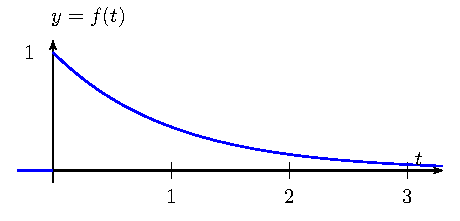
\includegraphics{cap_transformada_de_fourier/pics/figura_8}\end{center}
\begin{eqnarray*}
F(w)=\mathcal{F}\{f(t)\}&=&\int_{-\infty}^\infty f(t) e^{-i w t}dt\\
&=&\int_{0}^\infty e^{-at} e^{-i w t}dt\\
&=&\int_{0}^\infty e^{-at} \left(\cos(wt)-i\sen(wt)\right)dt\\
&=&\frac{a}{a^2+w^2}-\frac{iw}{a^2+w^2}\\
\end{eqnarray*}
onde se usou os itens 1 e 2 da tabela \ref{tab_int_def}.
\end{Answer}
\begin{Exercise}{\label{Exer_trans_exp_t2}} Considere a função $f(t)=e^{-at^2}$ onde $a$ é uma constante positiva. Trace o gráfico de $f(t)$ e obtenha sua transformada de Fourier (use $a=1$ no gráfico).
\end{Exercise}
\begin{Answer}
\begin{center}

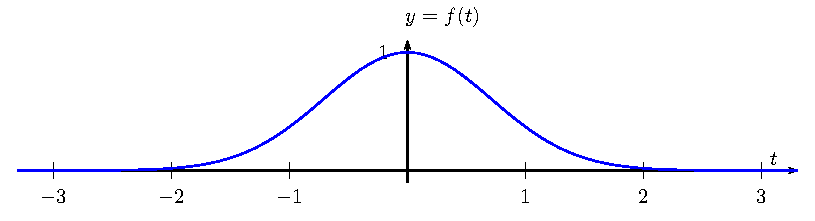
\includegraphics{cap_transformada_de_fourier/pics/figura_9}\end{center}
\begin{eqnarray*}
F(w)=\mathcal{F}\{f(t)\}&=&\int_{-\infty}^\infty f(t) e^{-i w t}dt\\
&=&\int_{-\infty}^\infty e^{-at^2} e^{-i w t}dt\\
&=&\int_{-\infty}^\infty e^{-at^2} \left(\cos(wt)-i\sen(wt)\right)dt\\
&=&2\int_{0}^\infty e^{-at^2} \cos(wt)dt\\
&=&\frac{\sqrt{\pi}}{\sqrt{a}}e^{-\frac{w^2}{4a}}
\end{eqnarray*}
onde se usou o item 8 da tabela \ref{tab_int_def}.
\end{Answer}
\begin{Exercise} {\label{ex_trans_Fou_0}}Calcule a transformada inversa da função $F(w)=\delta(w-w_0)+\delta(w+w_0)$
\end{Exercise}
\begin{Answer} $f(t)=\frac{1}{\pi}\cos(w_0t)$
\end{Answer}
\begin{Exercise}{\label{ex_inv_exp_kk}} Calcule a transformada inversa da função $F(k)=e^{-k^2}$
\end{Exercise}
\begin{Answer} $f(x)=\frac{1}{2\sqrt{\pi}} e^{-\frac{x^2}{4}}$
\end{Answer}
\begin{Exercise} Mostre que se $f(t)$ é uma função real par, então sua transformada de Fourier é uma função real.
\end{Exercise}
\begin{Exercise} Mostre que se $f(t)$ é uma função real ímpar, então sua transformada de Fourier é uma função imaginária.
\end{Exercise}
\begin{Exercise} Mostre que se $f(t)$ é uma função real, então sua a parte real da tranformada de Fourier de $f(t)$ é uma função par e a parte imaginária é ímpar.
\end{Exercise}
\begin{Exercise} Calcule a transformada de Fourier da função
$$f(t)=\sum_{j=0}^\infty \delta(t-j) e^{-j}.$$
\end{Exercise}
\begin{Answer} 
\begin{eqnarray*}
F(w)=\mathcal{F}\{f(t)\}&=&\int_{-\infty}^\infty f(t) e^{-i w t}dt\\
&=&\int_{-\infty}^\infty \left[\sum_{j=0}^\infty\delta(t-j)e^{-j}\right] e^{-i w t}dt\\
&=&\sum_{j=0}^\infty\int_{-\infty}^\infty \delta(t-j)e^{-j} e^{-i w t}dt\\
&=&\sum_{j=0}^\infty e^{-j} e^{-i w j}
=\sum_{j=0}^\infty e^{-(1+i w) j}\\
&=&\frac{1}{1-e^{-(1+i w)}}=\frac{1}{1-e^{-1}\left(\cos(w)-i\sen(w)\right)}\\
&=&\frac{1}{1-e^{-1}\cos(w)+ie^{-1}\sen(w)}\\
&=&\frac{1-e^{-1}\cos(w)+ie^{-1}\sen(w)}{\left(1-e^{-1}\cos(w)\right)^2+e^{-2}\sen^2(w)}\\
&=&\frac{1-e^{-1}\cos(w)+ie^{-1}\sen(w)}{1-2e^{-1}\cos(w)+e^{-2}}\\
\end{eqnarray*}
\end{Answer}
